% Institute of Computer Science thesis template
% authors: Sven Laur, Liina Kamm
% last change Tõnu Tamme 09.05.2017
%--
% Compilation instructions:
% 1. Choose main language on line 55-56 (English or Estonian)
% 2. Compile 1-3 times to get references right
% pdflatex bachelors-thesis-template
% bibtex bachelors-thesis-template
%--
% Please use references like this:
% <text> <non-breaking-space> <cite/ref-command> <punctuation>
% This is an example~\cite{example}.

\documentclass[12pt]{article}

% A package for setting layout and margins for your thesis 
\usepackage[a4paper]{geometry}

%%=== A4 page setup ===
%\setlength{\paperwidth}{21.0cm} 
%\setlength{\paperheight}{29.7cm}
%\setlength{\textwidth}{16cm}
%\setlength{\textheight}{25cm}


% When you write in Estonian then you want to use text with right character set
% By default LaTeX does not know what to do with õäöu letters. You have to specify
% a correct input and font encoding. For that you have to Google the Web     
%
% For TexShop under MacOS X. The right lines are 
%\usepackage[applemac]{inputenc}
%\usepackage[T1]{fontenc} %Absolutely critical for *hyphenation* of words with non-ASCII letters.
%
% For Windows and Linux the right magic lines are   
% \usepackage[latin1]{inputenc}
% \usepackage[latin5]{inputenc}
%%\usepackage[utf8]{inputenc} %Package inputenc Error: Unicode char ´ (U+B4) not set up for use with LaTeX
\usepackage[utf8x]{inputenc}
\usepackage[T1]{fontenc} %Absolutely critical for *hyphenation* of words with non-ASCII letters.

% Typeset text in Times Roman instead of Computer Modern (EC)
\usepackage{times}

% Suggested packages:
\usepackage{microtype}  %towards typographic perfection...
\usepackage{inconsolata} %nicer font for code listings. (Use \ttfamily for lstinline bastype)


% Use package babel for English or Estonian 
% If you use Estonian make sure that Estonian hyphenation is installed 
% - hypen-estonian or eehyp packages
%
%===Choose the main language in thesis
\usepackage[english]{babel} %the thesis is in English 

% If you have problems with Estonian keywords in the bibliography
%\usepackage{biblatex}
%\usepackage[backend=biber]{biblatex}
%\usepackage[style=alphabetic]{biblatex}
% plain --> \usepackage[style=numeric]{biblatex}
% abbrv --> \usepackage[style=numeric,firstinits=true]{biblatex}
% unsrt --> \usepackage[style=numeric,sorting=none]{biblatex}
% alpha --> \usepackage[style=alphabetic]{biblatex}
%\DefineBibliographyStrings{estonian}{and={ja}}
%\addbibresource{bachelor-thesis.bib}


% General packages for math in general, theorems and symbols 
% Read ftp://ftp.ams.org/ams/doc/amsmath/short-math-guide.pdf for further information
\usepackage{amsmath} 
\usepackage{amsthm}
\usepackage{amssymb}

% Optional calligraphic fonts    
% \usepackage[mathscr]{eucal}

% Print a dot instead of colon in table or figure captions
\usepackage[labelsep=period]{caption}

% Packages for building tables and tabulars 
\usepackage{array}
\usepackage{tabu}   % Wide lines in tables
\usepackage{xspace} % Non-eatable spaces in macros

% Including graphical images and setting the figure directory
\usepackage{graphicx}
\graphicspath{{figures/}}

% Packages for getting clickable links in PDF file
%\usepackage{hyperref}
\usepackage[hidelinks]{hyperref} %hide red (blue,green) boxes around links
\usepackage[all]{hypcap}


% Packages for defining colourful text together with some colours
\usepackage{color}
\usepackage{xcolor} 
%\definecolor{dkgreen}{rgb}{0,0.6,0}
%\definecolor{gray}{rgb}{0.5,0.5,0.5}
\definecolor{mauve}{rgb}{0.58,0,0.82}


% Standard package for drawing algorithms
% Since the thesis in article format we must define \chapter for
% the package algorithm2e (otherwise obscure errors occur) 
\let\chapter\section
\usepackage[ruled, vlined, linesnumbered]{algorithm2e}

% Fix a  set of keywords which you use inside algorithms
\SetKw{True}{true}
\SetKw{False}{false}
\SetKwData{typeInt}{Int}
\SetKwData{typeRat}{Rat}
\SetKwData{Defined}{Defined}
\SetKwFunction{parseStatement}{parseStatement}


% Nice todo notes
\usepackage{todonotes}

% comments and verbatim text (code)
\usepackage{verbatim}


% Proper way to create coloured code listings
\usepackage{listings}
\lstset{ 
  %language=python,                % the language of the code
  language=C++,
  basicstyle=\footnotesize,        % the size of the fonts that are used for the code
  %numbers=left,                   % where to put the line-numbers
  %numberstyle=\footnotesize,      % the size of the fonts that are used for the line-numbers
  numberstyle=\tiny\color{gray}, 
  stepnumber=1,                    % the step between two line-numbers. If it's 1, each line 
                                   % will be numbered
  numbersep=5pt,                   % how far the line-numbers are from the code
  backgroundcolor=\color{white},   % choose the background color. You must add \usepackage{color}
  showspaces=false,                % show spaces adding particular underscores
  showstringspaces=false,          % underline spaces within strings
  showtabs=false,                  % show tabs within strings adding particular underscores
  frame = lines,
  %frame=single,                   % adds a frame around the code
  rulecolor=\color{black},		   % if not set, the frame-color may be changed on line-breaks within 
                                   % not-black text (e.g. commens (green here))
  tabsize=2,                       % sets default tabsize to 2 spaces
  captionpos=b,                    % sets the caption-position to bottom
  breaklines=true,                 % sets automatic line breaking
  breakatwhitespace=false,         % sets if automatic breaks should only happen at whitespace
  %title=\lstname,                 % show the filename of files included with \lstinputlisting;
                                   % also try caption instead of title
  keywordstyle=\color{blue},       % keyword style
  commentstyle=\color{dkgreen},    % comment style
  stringstyle=\color{mauve},       % string literal style
  escapeinside={\%*}{*)},          % if you want to add a comment within your code
  morekeywords={*,game, fun}       % if you want to add more keywords to the set
}


% Obscure packages to write logic formulae and program semantics
% Unless you do a bachelor thesis on program semantics or static code analysis you do not need that
% http://logicmatters.net/resources/ndexamples/proofsty3.html <= writing type rules => use semantic::inference
% ftp://tug.ctan.org/tex-archive/macros/latex/contrib/semantic/semantic.pdf
\usepackage{proof}
\usepackage{semantic} 
\setlength{\inferLineSkip}{4pt}
\def\predicatebegin #1\predicateend{$\Gamma \vdash #1$}

% If you really want to draw figures in LaTeX use packages tikz or pstricks
% However, getting a corresponding illustrations is really painful  


% Define your favorite macros that you use inside the thesis 
% Name followed by non-removable space
\newcommand{\proveit}{ProveIt\xspace}

% Macros that make sure that the math mode is set
\newcommand{\typeF}[1] {\ensuremath{\mathsf{type_{#1}}}\xspace}
\newcommand{\opDiv}{\ensuremath{\backslash \mathsf{div}}\xspace} 

% Nice Todo box
\newcommand{\TODO}{\todo[inline]}

% A way to define theorems and lemmata
\newtheorem{theorem}{Theorem}



%%% BEGIN DOCUMENT
\begin{document}

%===BEGIN TITLE PAGE
\thispagestyle{empty}
\begin{center}

\large
UNIVERSITY OF TARTU\\%[2mm]
Institute of Computer Science\\
Software Engineering Curriculum\\%[2mm]

%\vspace*{\stretch{5}}
\vspace{25mm}

\Large Jaan Tohver

\vspace{4mm}

\huge Optical Character Recognition for Extremely Low Quality Images

%\vspace*{\stretch{7}}
\vspace{20mm}

\Large Master's Thesis (30 ECTS)

\end{center}

\vspace{2mm}

\begin{flushright}
 {
 \setlength{\extrarowheight}{5pt}
 \begin{tabular}{r l} 
  \sffamily Supervisor: & \sffamily Gholamreza Anbarjafari, PhD
 \end{tabular}
 }
\end{flushright}

%\vspace*{\stretch{3}}
%\vspace{10mm}

\vfill
\centerline{Tartu 2018}

%===END TITLE PAGE

% If the thesis is printed on both sides of the page then 
% the second page must be must be empty. Comment this out
% if you print only to one side of the page comment this out
%\newpage
%\thispagestyle{empty}    
%\phantom{Text to fill the page}
% END OF EXTRA PAGE WITHOUT NUMBER


%===COMPULSORY INFO PAGE
\newpage

%=== Info in English
\noindent\textbf{\large Optical Character Recognition for Extremely Low Quality Images}

\vspace*{3ex}

\noindent\textbf{Abstract:}\\

Optical character recognition (OCR) from printed and handwritten documents is a solved problem for all practical purposes. Modern OCR systems are able to achieve a 99.9\% detection rate which is on par with human capabilities. Where most OCR systems fall short is when the input is of low quality, such as containing large amounts of noise or motion blur, or being of low resolution.

A real world use-case of this problem is detecting car licence plates from a security camera feed. Security cameras are often of low resolution, use high levels of compression, and have low framerate since the video footage needs to be stored for a long period of time and storage cost is paramount. In addition, cars can move unpredictably causing motion blur during the capture of a video frame.

The goal of this project is to test various methods of improving OCR accuracy with low quality input. Namely,
\begin{itemize}
  \item Training a neural network (NN) on low quality images and testing results on low quality images.
  \item Training a NN on high quality images and testing on digitally enhanced low quality images.
  \item Training a NN on digitally enhanced low quality images and testing on digitally enhanced images.
  \item Using multiframe registration of frames from a video feed to improve detection quality.
\end{itemize}

The tests will be conducted using frames from a blurry, noisy, and low resolution video feed containing text. Third party solutions are used to extract areas containing text from those frames.

Some of the training and test data is gathered specifically for this task by filming, and extracting frames from an intentionally blurry video. Additional synthetic motion blur is added to some of the images. Some data is gathered from available open source databases, such as images containing vehicle licence plates.

\vspace*{1ex}

\noindent\textbf{Keywords:}\\

OCR, Deblurring, Low Quality, Low Resolution

%Layout, formatting, template

\vspace*{1ex}

\noindent\textbf{CERCS:}\\

\TODO{CERCS code and name:~\url{https://www.etis.ee/Portal/Classifiers/Details/d3717f7b-bec8-4cd9-8ea4-c89cd56ca46e}}

\vspace*{1ex}

\newpage

\tableofcontents

% Remember to remove this from the final thesis version
\newpage
\listoftodos[Unsolved issues]
% END OF TODO PAGE 


\newpage
\section{Introduction}

Optical character recognition (OCR) is the conversion of text to a machine encoded form, such as converting images or printed documents to text documents. OCR is not a new concept by any means. A patent for a system which can be called the predecessor of modern OCR was already granted in 1931~\cite{1838389}. Modern OCR systems are, of course, far more powerful.

\subsection{Motivation}

For all intents and purposes OCR is basically a solved problem for detecting text from clear and high resolution images containing printed or handwritten text. Modern systems perform on par with human capabilities in this regard, boasting a 99.9\% detection rate. A problem still being researched, however, is OCR from low quality images. Low quality can mean low resolution, high levels of compression, containing artefacts generated by scanning or image capture, containing motion blur caused by the movement of the subject or the camera during image capture, or any combination thereof.

Accurate OCR from low quality images and video could solve several problems for automating processes where the system needs to detect some text. For example in an autonomous parking garage, where a camera is filming approaching cars, a system analyses the video feed and opens the gate or barrier for cars with licence plate numbers matching authorized users.

\subsection{Contributions}

The goal of this thesis is to test different approaches for such a system. Namely,
\begin{itemize}
  \item Training a neural network (NN) on low quality images and testing results on low quality images.
  \item Training a NN on high quality images and testing on digitally enhanced low quality images.
  \item Training a NN on digitally enhanced low quality images and testing on digitally enhanced images.
  \item Using multiframe registration of frames from a video feed to improve detection quality.
\end{itemize}

Neural networks behave in very specific ways in regards to the data that was used for training them. Understanding how image enhancement and OCR networks behave under such conditions gives valuable insight into which training data to use to improve OCR accuracy for low quality images while also retaining accuracy for high resolution and high quality images.

\TODO{Add accurate contribution after work is done.}

\subsection{Outline}

The thesis is structured as follows.

\noindent
\textbf{Chapter 2} describes both the history and the state of the art in OCR and low quality image enhancement and discusses the advantages and drawbacks of each of the approaches.\\
\textbf{Chapter 3} describes the research problem and the necessity of finding a solution to the problem.\\
\textbf{Chapter 4} describes in detail the approach taken to solve the problem.\\
\textbf{Chapter 5} describes the evaluation process of the results as well as a comparison to related work.\\
\textbf{Chapter 5} concludes the thesis with a summary and research directions for the future

\newpage
\section{Background}

This section gives an overview of the history of OCR and image enhancement solutions as well as research and commercial products related to the topic.

\subsection{History}

\subsubsection{OCR}

The history of OCR can be traced back to the late 1920s when the inventor Emanuel Goldberg started developing a system called "Statistical Machine" which searched microfilm archives using an optical code recognition system. He was granted a patent for his invention in 1931, which was later acquired by IBM~\cite{1838389}.

\subsubsection{Digital Image Enhancement}

Digital image enhancement has been around for as long as digital images have i.e., since the 1950s~\cite{dipanniversary}. In essence a very simple concept - take the pixel values of an image and, using some algorithm, modify them to produce a clearer image. It was advanced further alongside astronomical and medical research~\cite{Rosenfeld}.

\subsection{State of the Art}

\subsubsection{Neural Networks}

Most modern OCR systems and image enhancement techniques are based on artificial neural networks, often called just neural networks (NNs). Which makes this a necessity is the fact that both of those problems are very dynamic and not well solvable algorithmically.

The theoretical base for NNs dates back to the end of the 1800s and is based on the structure of the human brain in which neurons interact with each other and the bonds between neurons can strengthen and weaken over time~\cite{SCHMIDHUBER201585}.

An artificial neural network consists of many simple connected processors, called artificial neurons, which produce activations based on an activation function producing real numbers in a predefined range. The simplest neural network consists of an input layer and an output layer. The neurons in the input layer produce activations based on the input. The output layer produces an output based on the activations of input layers~\cite{SCHMIDHUBER201585}.

Most NNs are not as simple as that and contain any number of hidden layers between the input and output layers. These hidden layers consist of any number of neurons which produce activations based on the output of another layer. There are various architectures used for NNs, some are combinations of other types of networks. This work mostly focuses on convolutional neural networks (CNNs) and recurrent neural networks (RNNs)~\cite{SCHMIDHUBER201585}.

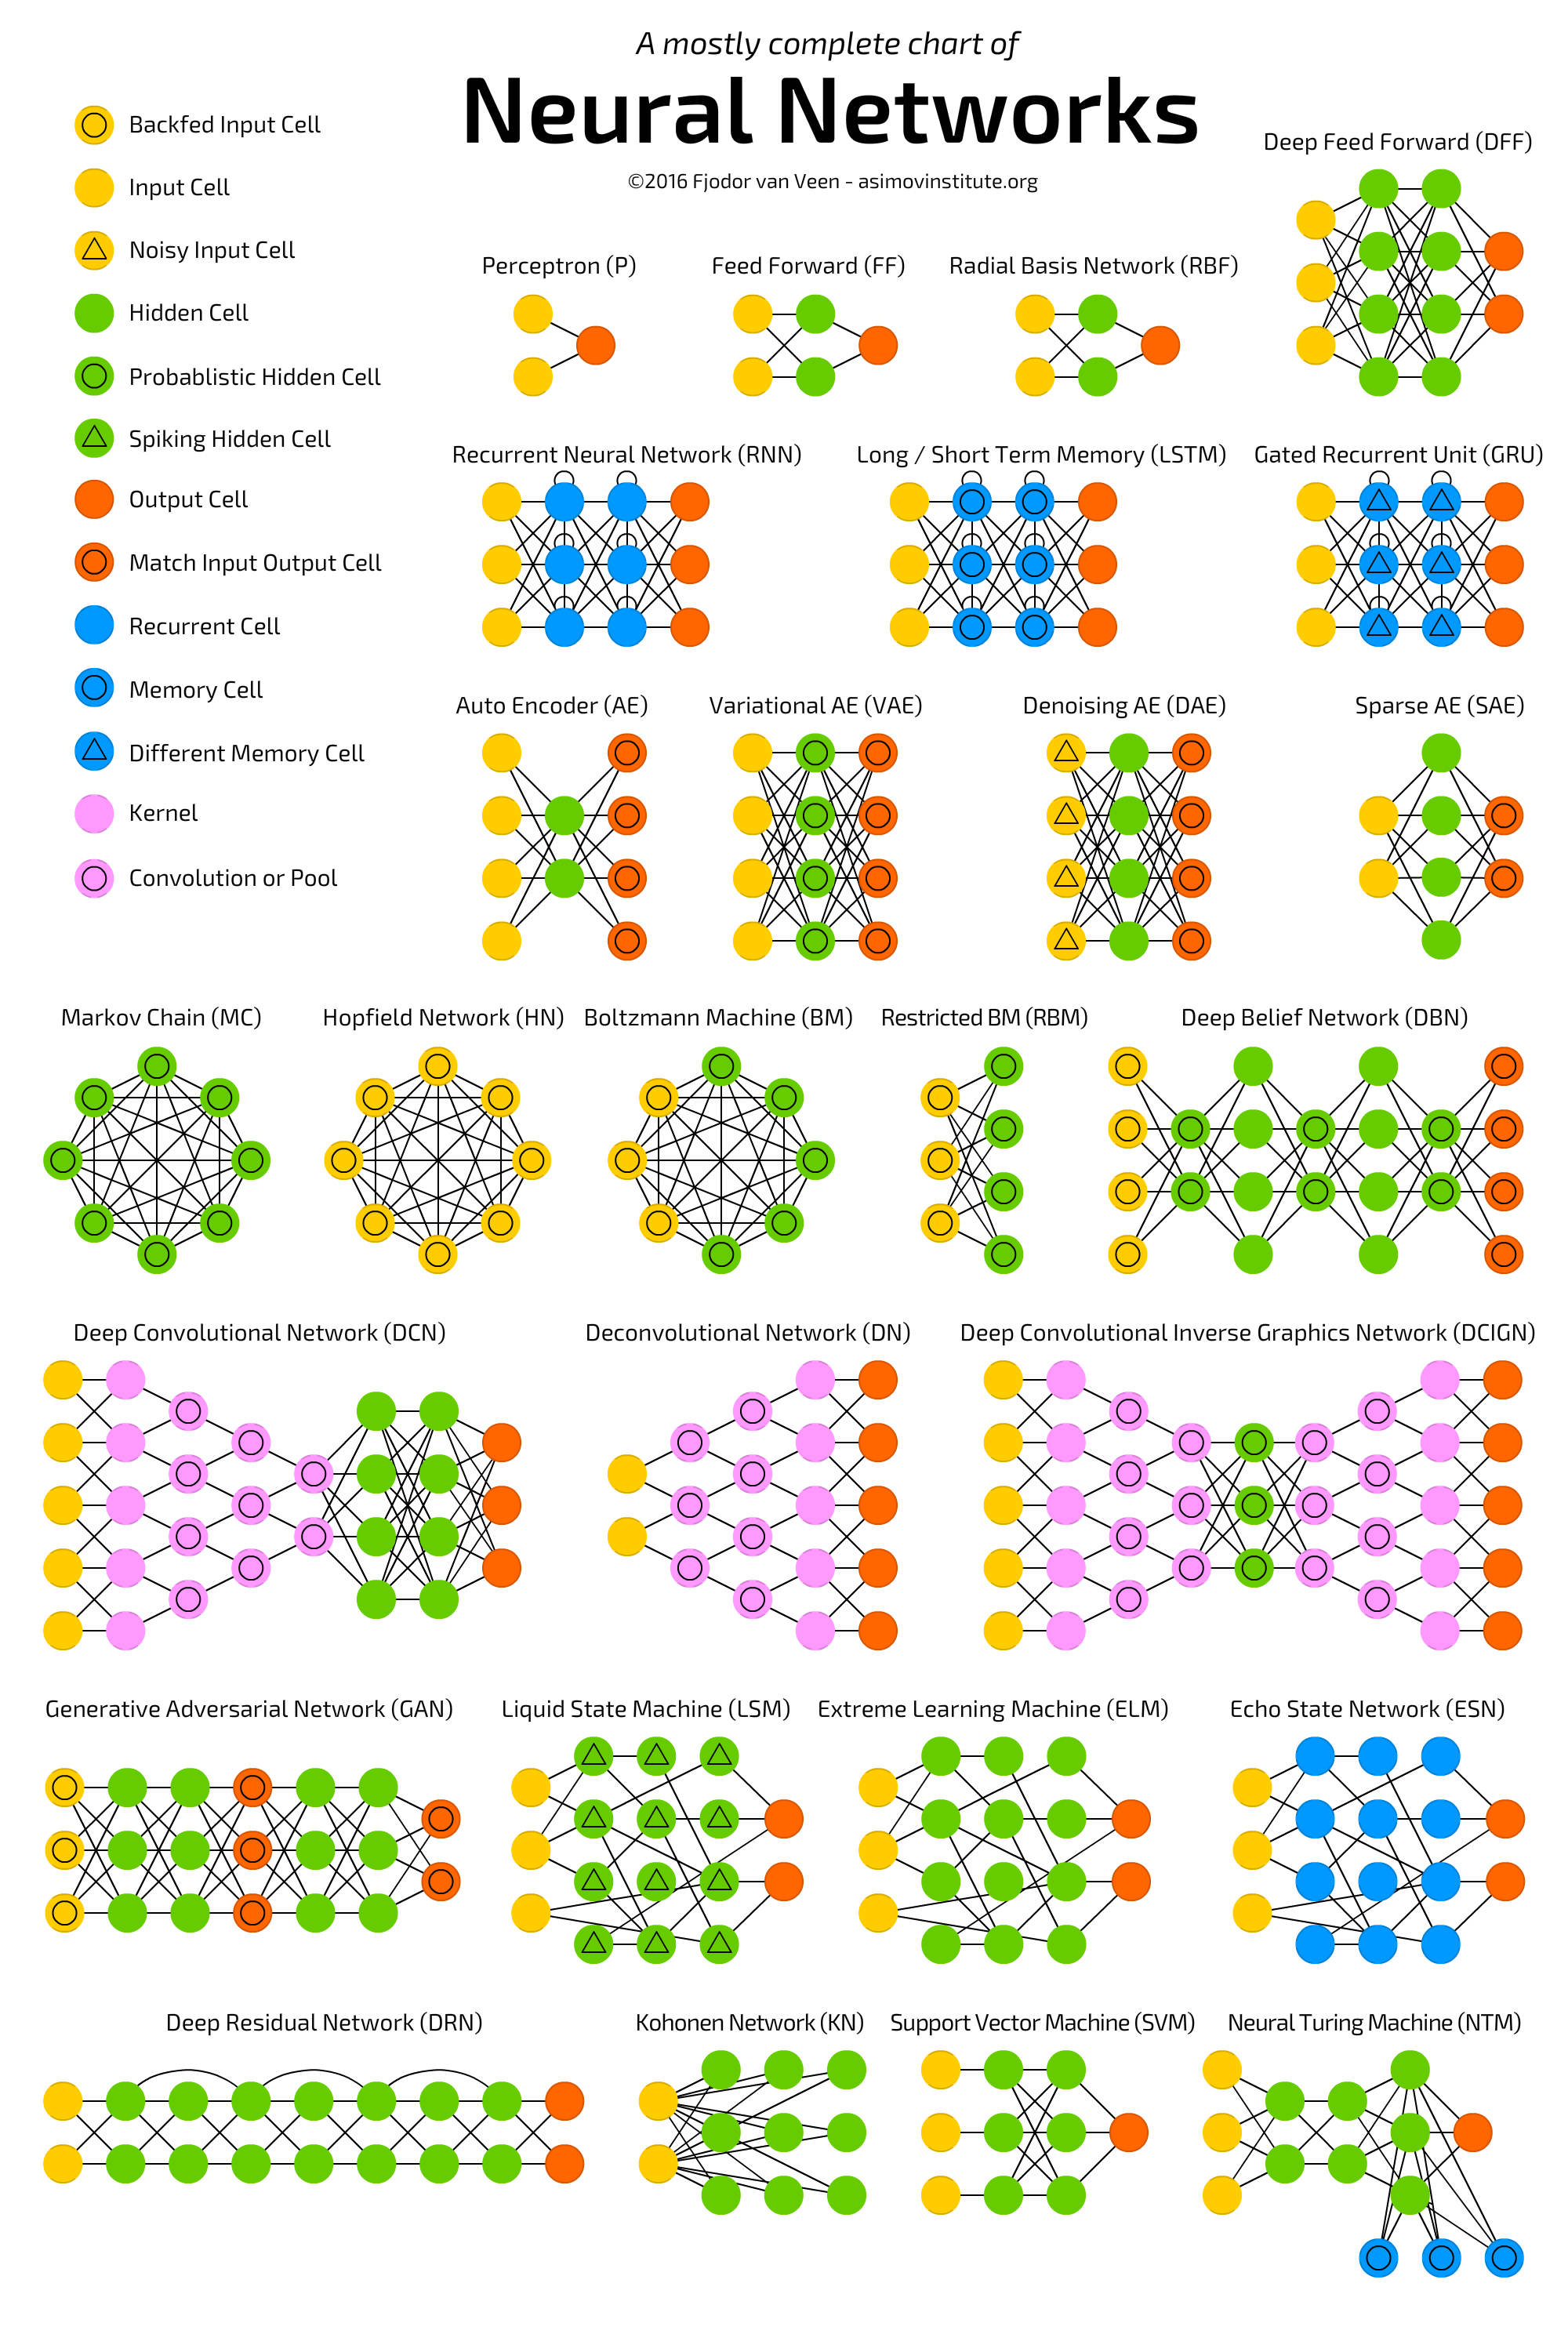
\includegraphics [width=\textwidth, height=\textheight, keepaspectratio] {neuralnetworks.png}~\cite{netzoo}

CNNs are primarily used for image processing. CNNs are feedforward networks (FFNs), which means that neurons do no back-propagate any information and only pass it forward to the next layer. A distinct feature of CNNs is that they consist of convolutional layers in which not all neurons are connected to all neurons in the previous and next layers~\cite{SCHMIDHUBER201585}.

RNNs are primarily used for text and speech processing. RNNs are FFNs like CNNs. However, unlike CNNs they are stateful, meaning that in addition to receiving data from the previous layer, each neuron retains data from previous passes. RNNs are also able to handle arbitrary input and output lengths unlike CNNs~\cite{SCHMIDHUBER201585}.

\TODO{1979: convolution + weight replication + subsampling (Neocognitron)}

\subsubsection{OCR}

OCR is a difficult problem since a sufficiently dynamic OCR system should be able to work on hundreds of different scripts containing tens of millions of different characters. As it stands, OCR systems are quite specific to a problem they solve, such that moving from latin script to an urdu script is a difficult task for an OCR system~\cite{urdu}.

Many OCR engines support over 100 languages, such as Tesseract, probably the most well known one. It started as proprietary software developed by Hewlett Packard in 1985, but was open sourced in 2005. Since then its development is continued by the community. Development has been sponsored by Google starting from 2006~\cite{tesseract}.

Still, it is not ideal that OCR systems have to be trained to fit specific requirements. An ideal system would be able to recognise characters from whichever character set it is given as input.

CNNs and RNNs are not mutually exclusive, however, and B. Shi et al devised one of the most promising novel OCR concepts in recent history in the form of a convolutional recurrent neural network (CRNN) in their 2015 paper "An End-to-End Trainable Neural Network for Image-based Sequence Recognition and Its Application to Scene Text Recognition"~\cite{Shi2017AnET}.

Their reasoning is that popular models like CNN cannot be applied to sequence prediction, since they operate on fixed size inputs and outputs. CRNN then behaves like an RNN in that it can accept inputs and return outputs of arbitrary size, while still retaining properties of CNNs which make them invaluable in image processing~\cite{Shi2017AnET}.

\subsubsection{Digital Image Enhancement}

What makes digital image enhancement such a complicated research subject is the fact there is no agreed upon metric for measuring the performance of an image enhancement method. The results of a process such as image deblurring are largely subjective.

OCR is a very good context for measuring image enhancement, since the results, in this case OCR accuracy, are directly measurable before and after the enhancement process. M. D. Kim et al propose a quantitative method of measuring image deblurring accuracy in their paper "Dynamics-Based Motion Deblurring Improves the Performance of Optical
Character Recognition During Fast Scanning of a Robotic Eye". In addition, they note that computation time is extremely important to modern image processing solutions~\cite{dynbmd}. Indeed, since a lot of image processing happens in smartphones and microcomputers computational requirements are crucial in comparing image enhancement methods.

In point of fact, motion deblurring is very important for OCR overall. Especially with so many photos of documents taken. In 2005, already when smartphones were not as prevalent as they are today, Xing Yu Qi at al address this concern in their paper "Motion Deblurring for Optical Character Recognition" where they handle three types of image degradation - blurring, point wise nonlinearities, and additive noise. They do this by first determining the orientation and extent of the blurred area and then recovering it~\cite{1575575}.

Alongside the rising popularity of smartphones came the process of archiving documents by taking a photo. Scanning hardware has improved considerably since digitizing documents became popular. However, in the case of photos taken by smartphones, many of the original copies of the documents have been lost since and improving the quality of existing documents is the only way to restore their readability. J. Jiao et al propose a novel CNN based two-stage technique for document deblurring~\cite{8270051}.

A significant improvement of their approach, over previous approaches, is not requiring information about specifics of the style of the blurring for the image. They divide the image into sub-spaces and for each of those a corresponding degradative kernel space is developed. This solution not only works on different types of blurry images, but also on images that contain multiple types of blur, of which motion and focal blur are most prominent.~\cite{8270051}.

\clearpage
\section{Conclusion}

Outline from the template:
\TODO{What did you do?} 
\TODO{What are the results?}
\TODO{Future work?}

A paragraph or two about the results, including tables comparing different permutations of training data for networks.
\\\\
Future work in regards to additional image and video processing methods that can be utilized for this purpose.

\newpage

% BibTeX bibliography
\bibliographystyle{IEEEtran} %plain=[1], alpha=[BGZ09]
\bibliography{bachelor-thesis}

\addcontentsline{toc}{section}{\refname}

% Use Biblatex if you have problems with Estonian keywords
%\printbibliography %biblatex

% Use alternative local LaTeX bibliography
\begin{comment}
\begin{thebibliography}{9}
\bibitem{proVerif} 
  Bruno Blanchet. 
  Proverif: Cryptographic protocol verifier in the formal model.
  \url{http://www.proverif.ens.fr/}.
  (checked 15.05.2012)
\bibitem{GameB_1} GameB1
\bibitem{GameB_2} GameB2
\bibitem{certicrypt} certicrypt
\bibitem{kamm12} kamm12
\end{thebibliography}
\end{comment}


\newpage

{\section*{Appendix}
  \addcontentsline{toc}{section}{Appendix}
}

\newpage

\section*{I. Glossary}
\addcontentsline{toc}{subsection}{I. Glossary}

\newpage

\section*{II. Licence}

\addcontentsline{toc}{subsection}{II. Licence}

\subsection*{Non-exclusive licence to reproduce thesis and make thesis public}

I, \textbf{Jaan Tohver},

\begin{enumerate}
\item
herewith grant the University of Tartu a free permit (non-exclusive licence) to:
\begin{enumerate}
\item[1.1]
reproduce, for the purpose of preservation and making available to the public, including for addition to the DSpace digital archives until expiry of the term of validity of the copyright, and
\item[1.2]
make available to the public via the web environment of the University of Tartu, including via the DSpace digital archives until expiry of the term of validity of the copyright,
\end{enumerate}

of my thesis

\textbf{Optical Character Recognition for Extremely Low Quality Images}

supervised by Gholamreza Anbarjafari, PhD

\item
I am aware of the fact that the author retains these rights.
\item
I certify that granting the non-exclusive licence does not infringe the intellectual property rights or rights arising from the Personal Data Protection Act. 
\end{enumerate}

\noindent
Tartu, 16.12.2018

\end{document}